\section{Algorithm}
\label{sec:algorithm}

In this section, we describe the steps of our instance-based
POS-induction algorithm:
\begin{enumerate}
  \item Sample $r$ substitutes for each word instance in the target
    corpus using an n-gram language model.
  \item Construct $r$ tuples for each instance where each tuple
    consists of a sampled substitute, the target word, and the
    morphological and orthographical features of the target word (see
    Table~\ref{tab:sampleswithfeatures}).
  \item Construct Euclidean embeddings of each word and each feature based on
    all tuples following Gleberson et al.\shortcite{globerson2007euclidean}
    and Maron et al.\shortcite{maron2010sphere}.
  \item Construct a vector representation for each instance by
    concatenating the embedding of the target word with the average of
    its substitute embeddings.
  \item Use $k$-means clustering to cluster the instance vectors where
    $k$ is equal to the number of gold tags.
  %% \item Construct a mapping from clusters to tags for evaluation using
  %%   the most frequent tag found in each cluster.
\end{enumerate}

Steps 1 and 2 construct a tuple representation for each instance.
Table~\ref{tab:sampleswithfeatures} gives some example tuples for Sentence (1)
from the previous section.  In this example $r=3$, so three substitutes are
sampled for each instance as contextual features.  The sampling is with
replacement from the substitute word distribution of a context given by the
n-gram language model, so some substitute words may be repeated.  The target
word and its other features are identical for each of the $r$ tuples
representing a single instance.

\begin{table}[t]
  \centering
  \begin{tabular}{|lllll|}
    \hline
    {\bf Word} & {\bf Subst} & {\bf Suf} & {\bf Cap} & {\bf Num} \\
    \hline
    Vinken & Makhlouf & -- & T & F\\
    Vinken & Makhlouf & -- & T & F\\
    Vinken & \unk & -- & T & F\\
    61 & 20 & -- & F & T\\
    61 & 2000 & -- & F & T\\
    61 & eleven & -- & F & T\\
    years & years & -s & F & F\\
    years & years & -s & F & F\\
    years & years & -s & F & F\\
    \hline
  \end{tabular}
  \caption{The tuples constructed for the instances of ``Vinken'',
    ``61'' and ``years'' from Sentence (1).  The elements of each tuple
    are the target word, sampled substitute, suffix, capitalization, and
    number features.}
  \label{tab:sampleswithfeatures}
\end{table}

%% We construct the co-occurrence data as word--features tuples that consist of
%% word, and its contextual (substitutes), orthographic and morphological
%% features.  Contextual features are sampled from the substitute word
%% distribution of the instance context.  If $r$ random substitutes are sample for
%% each instance than there will be $r$ identical tuples except the contextual
%% features.  Table~\ref{tab:sampleswithfeatures} presents the co-occurrence
%% tuples of each instance in a sample sentence when $r$ is equal to 1.  

%% \begin{table*}[!t]
%%   \centering
%%   \footnotesize
%% \begin{tabular}{|lllllll|}
%%   \hline
%%   \textbf{Word} & {\bf Contextual} & {\bf Morphology} &
%%   \specialcell{{\bf Initial}\\{\bf Capital}} & {\bf Number} &
%%   \specialcell{{\bf Contains}\\{\bf Hypen}} &
%%   \specialcell{{\bf Initial}\\{\bf Apostrophe}}
%%   \\
%%   \hline
%%   W:Pierre & \textit{C:Adrian} & & {\it F:IC} &&&\\
%%   W:Vinken & \textit{C:Danon} & & {\it F:IC} &&&\\
%%   W:, & \textit{C:\{} & & &&&\\
%%   W:61 & \textit{C:fourteen} & & & {\it F:N}&&\\
%%   W:years & \textit{C:years} & {\it F:s} &&&&\\
%% %%W:old & \textit{C:old} & & &&&\\
%% %%W:join & \textit{C:head} &&&&&\\
%% %%W:the & \textit{C:its} &&&&&\\
%% %%W:board & \textit{C:company} &&&&&\\
%% %%W:as & \textit{C:as} &&&&&\\
%% %%W:a & \textit{C:a} &&&&&\\
%% %%W:nonexecutive & \textit{C:non-executive} &&&&&\\
%% %%W:director & \textit{C:chairman} & {\it F:or}&&&&\\
%% %%W:Nov. & \textit{C:May} &&{\it F:IC}&&&\\
%% %%W:29 & \textit{C:9} &&&{\it F:N}&&\\
%% %%W. & \textit{C:.} & &&&&\\
%%   \hline
%% \end{tabular}
%% \caption{The first five words of the input sentence \textit{``Pierre Vinken, 61
%%   years old, will join the board as a nonexecutive director Nov.~29 .''} is
%%   represented with their contextual, orthographic and morphological features as
%%   tuples.  The leftmost column presents the target word, second column
%%   represents the contextual, third column is the morphological and the rest of
%%   the columns are the orthographic features.  Unobserved features are set to
%%   null.}
%% \label{tab:sampleswithfeatures}
%% \end{table*}

In step 3, we construct Euclidean embeddings for each unique word and
feature value using the multi-variable version of the CODE algorithm
described in \cite{globerson2007euclidean}.  Given two categorical
variables $X$ and $Y$, the CODE algorithm constructs Euclidean
embeddings (vectors) for each of their distinct values in the same
space.  The distance between an $x$ vector and a $y$ vector is related
to their joint distribution $p(x, y)$ as
follows\footnote{\cite{globerson2007euclidean} describes several ways
  to relate distances to probabilities, the model used here is the
  marginal-marginal (MM) model.}

\[ p(x,y) = \frac{1}{Z} \bar{p}(x) \bar{p}(y) e^{-d^2_{x,y}} \]

\noindent where $\bar{p}$ represents empirical probabilities
(frequencies from the training data), $d_{x,y}$ is the distance
between the embeddings of $x$ and $y$ and $Z=\sum_{x,y} \bar{p}(x)
\bar{p}(y) e^{-d^2_{x,y}}$ is a normalization constant.  Starting with
random vectors for each distinct value of $x$ and $y$, we use
stochastic gradient ascent to move the embedding vectors around to
maximize the likelihood given by this model.  Calculating the
normalization constant $Z$ is the most expensive part of this
procedure.  We solve this problem following \cite{maron2010sphere} who
suggest that a constant $Z$ approximation can be used if the
embedding vectors are kept on the unit sphere.

As Table~\ref{tab:sampleswithfeatures} shows, considering the target
word and its contextual, morphological and orthographic features gives
us more than two variables.  Yatbaz et
al. \shortcite{yatbaz-sert-yuret:2012:EMNLP-CoNLL} adopt the two
variable CODE algorithm to this multi-variable case in an ad-hoc
manner by considering the target word as $x$ and all other features as
distinct $y$ values.  We implement the multi-variable extension of
CODE suggested by \cite{globerson2007euclidean} (Section 6.2) which
optimizes the following likelihood function:

\[ \ell(\phi, \psi^{(1)}, \ldots, \psi^{(K)}) = 
    \sum_{i=1}^K \sum_{w,f^{(i)}} \bar{p}(w,f^{(i)}) \log p(w,f^{(i)}) \]

\noindent where $\phi$ are the embeddings of target words, $\psi^{(i)}$ are the
embeddings for the values of the $i$'th feature $f^{(i)}$.  The set of
$K$ bivariate CODE models
$p(w,f^{(i)})$ share the same target word embeddings $\phi(w)$ but
build their own feature embeddings $\psi^{(i)}(f^{(i)})$.

%% To handle co-occurrence tuples we use the modified version of S-CODE that can
%% model more than two variables (see Appendix~\ref{app:multiscode}).  We feed
%% the tuples to the modified S-CODE which places $n$-dimensional embeddings for
%% word types that frequently co-occur with the same features (and features that
%% co-occur with the same words types) close to each other on the sphere.
%% Figure~\ref{fig:scodeexample} illustrates the embeddings of a sample
%% co-occurrence data on a sphere after S-CODE converges.  This modified S-CODE is
%% aware of the feature types which enables us to construct our instance based
%% representation.  In addition, the modified S-CODE can weight the different
%% feature types and this will be the interest of future work. 

%% \begin{figure}[h]
%% \centering
%%  \begin{minipage}[c]{0.49\columnwidth}
%%   \footnotesize
%%   \begin{tabular}{l|l}
%%     \textbf{Word} & \textbf{Substitute} \\
%%     \hline
%%     $\hdots$&$\hdots$\\
%%     W:director & S:chairman \\
%%     W:chief & S:chairman \\
%%     $\hdots$&$\hdots$\\
%%     W:Pierre & S:John \\
%%     W:Frank & S:John \\
%%     $\hdots$&$\hdots$\\
%%   \end{tabular}
%%   \end{minipage} \hfill
%%   \begin{minipage}[c]{0.49\columnwidth}
%%     \raisebox{-\height}{
%%       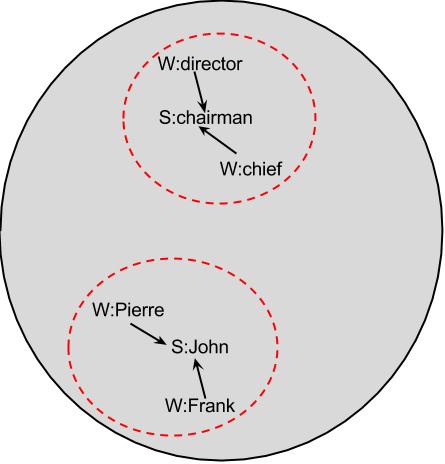
\includegraphics[width=1\columnwidth]{scode-ex.png}
%%     }
%%   \end{minipage}
%%   \caption{The table on the left is a co-occurrence data and  figure on the
%%   right represents the final embeddings of the words and contextual features
%%   after S-CODE converges.  Dashed circles represent the possible groupings of the
%%   word type embeddings on the sphere.}
%%   \label{fig:scodeexample}
%% \end{figure}

%The limitation of representing co-occurrence data as pairs is that S-CODE can
%not distinguish whether the type of the word-feature pair is contextual,
%orthographic or morphological.  

Step 4 constructs a vector representation for each word instance with the
concatenation of its word type embedding and the average of its $r$ substitute
embeddings.  If the original embeddings are in $d$ dimensional space, this
results in a $2d$ dimensional vector representing an instance.

Step 5 clusters these $2d$ dimensional instance vectors using a
modified k-means algorithm with smart initialization
\cite{arthur2007k} and assigns each instance to one of $k$ clusters.
%% Step 6 constructs a mapping between the clusters and the gold tags
%% for evaluation.  

%% Yatbaz et al.\shortcite{yatbaz-sert-yuret:2012:EMNLP-CoNLL} model co-occurrence
%% pairs using the S-CODE with two variables and cluster the embeddings of word
%% types with weighted k-means algorithm.  The sentences in
%% Figure~\ref{fig:typelimitation} illustrates the limitation of clustering word
%% type embeddings.  The word {\em offer} is a {\em verb} in the first sentence
%% and a {\em noun} in the second one.  S-CODE constructs only one embedding for
%% each unique word type and feature value.  Thus clustering the word type
%% embeddings is actually applying the one-tag-per-word assumption.

%% \begin{figure}[ht]
%%   %  \begin{minipage}[c]{\columnwidth}
%%     \begin{tabular}{ll}
%%       (1) & $\hdots$ it will also {\em offer} buyers the option $\hdots$\\
%%       &{\bf Substitutes:} give, help, attract\\ 
%%       (2) & The {\em offer} is being launched $\hdots$\\ 
%%       &{\bf Substitutes:} campaign, project, scheme\\ 
%%     \end{tabular}
%%    \caption{Ambiguous occurrences of the word {\em offer}.}
%%    \label{fig:typelimitation}
%%    %\end{minipage} \hfill
%%  \end{figure}
%% On the other hand, the substitutes of {\em offer} in both of the sentences can
%% semantically and syntacticly disambiguates the correct category of the
%% corresponding occurrences.  

%% The next section presents the results of our system and compares them with the
%% results of the word based state-of-the-art system. 
%% To construct the co-occurrence data we pair each word instance with randomly
%% sampled substitutes that can be observed in the context of the corresponding
%% instance and with orthographic and morphological features of the word instance.
%% Random substitutes were sampled (with replacement) from a substitute word
%% distribution for the context calculated based on an n-gram language model.  
%% 
%% We enriched the word--substitute co-occurrence data by extracting morphological
%% and orthographic features and incorporating them as word--feature pairs.  They
%% fed the co-occurrence data into the S-CODE algorithm.  S-CODE places the
%% embeddings for word types that frequently co-occur with the same substitutes or
%% features (and substitutes or features that co-occur with the same words) close
%% to each other on the $n$-dimensional sphere.  Finally, they apply k-means
%% clustering to group vectors of word types to induce word categories.
%% 
%% First, we construct a pairwise co-occurrence
%% representation of words and their substitutes.  Next, we map each word and each
%% substitute in the co-occurrence data to real vectors (embeddings) on an
%% $n$-dimensional sphere using the S-CODE algorithm \cite{maron2010sphere}.
%% S-CODE places the vectors for words that frequently co-occur with the same
%% substitutes (and substitutes that co-occur with the same words) close to each
%% other on the sphere.  We then construct vectors for each word instance by using
%% the embeddings of the word itself and its sampled substitutes in the
%% co-occurrence data.  Finally, we apply k-means clustering to group these
%% vectors to induce word categories.  
%% 
%% In Section~\ref{sec:cooc} we detail the representation of words and their
%% substitutes as co-occurrence data, in Section~\ref{sec:embedding} we describe
%% the embedding algorithm, and finally Section~\ref{sec:clustering} describes how
%% we represent the word instances using the embeddings calculate in the previous
%% step.
%% 
%% \subsection{Context Representation}
%% \label{sec:cooc}
%% % How we represent the context?
%% % How we relate the word and the context?
%% 
%% We represent the context of a word with random substitutes that are
%% likely to occupy the same position as the word.  We sample random
%% substitutes (with replacement) from a substitute word distribution for
%% the context calculated based on an n-gram language model.  The sample
%% space of the substitute word distribution is the vocabulary of the
%% language model.
%% %% \footnote{Sampled substitutes might include the unknown
%% %%   word tag \unk\ representing words outside the fixed size
%% %%   vocabulary of the language model.  For example proper nouns
%% %%   typically have \unk\ as a substitute.}  
%% In effect, we are using substitute word distributions and the sampled random
%% substitutes as {\em contextual features} that represent properties of a word's
%% position.  Table~\ref{tab:subdist} shows the substitute word distributions for
%% some positions in an example sentence.
%% %% \begin{table*}[t]
%% %%   \footnotesize
%% %%   \centering
%% %%   \caption{The substitute word distributions (with probabilities in
%% %%     parentheses) for some of the positions in the example sentence
%% %%     \textit{``Pierre Vinken, 61 years old, will join the board as a
%% %%     nonexecutive director Nov.~29.''} based on a 4-gram language
%% %%   model.}
%% %%   \label{tab:subdist}
%% %%   \begin{tabular}{|ll|} \hline
%% %%     \textbf{will:} & \textit{will} (0.9985), \textit{would} (0.0007), \textit{to} (0.0006), \textit{also} (0.0001), $\ldots$ \\
%% %%     \textbf{join:} & \textit{join} (0.6528), \textit{leave} (0.2140), \textit{oversee} (0.0559), \textit{head} (0.0262), \textit{rejoin} (0.0074), $\ldots$ \\
%% %%     \textbf{the:}  &\textit{its} (0.9011), \textit{the} (0.0981), \textit{a} (0.0006), $\ldots$ \\
%% %%     \textbf{board:} & \textit{board} (0.4288), \textit{company} (0.2584), \textit{firm} (0.2024), \textit{bank} (0.0731), \textit{strike} (0.0030), $\ldots$ \\
%% %%     \hline
%% %%   \end{tabular}
%% %% \end{table*}
%% %%
%% To capture the relation between each word and its context we construct
%% a co-occurrence representation by pairing the words with randomly
%% sampled substitutes.  Table~\ref{tab:samples} shows random substitutes of each
%% word and their pairwise co-occurrence representation input to S-CODE on an
%% example sentence.  It is possible (and beneficial) to sample more than one
%% substitute and generate multiple pairs for the same word-context pair as seen
%% in Table~\ref{tab:samples}.  In the co-occurrence data, a target word might
%% appear both as a word and a random substitute therefore to clarify this
%% ambiguity we prepend ``W:'' and ``S:'' to words and substitutes, respectively.
%% The calculation of substitute distributions and substitute word sampling are
%% detailed in Appendix~A.
%% %% \begin{table}[h]
%% %%   \footnotesize
%% %%   \caption{The table on the left shows three possible substitutes
%% %%     sampled with replacement for each position in an example sentence
%% %%     based on a 4-gram language model.  The table on the right is the
%% %%     pairwise co-occurrence data fed to the S-CODE algorithm derived
%% %%     from these samples.  The prefixes ``W:'' and ``S:'' are used to
%% %%     distinguish target words and substitutes.  Sampled substitutes
%% %%     might include the unknown word tag ``\unk'' representing words
%% %%     outside the fixed size vocabulary of the language model.}
%% %% \begin{tabular}{|ll|} \hline
%% %% \textbf{Word} & \textbf{Random Substitutes}\\
%% %% \hline
%% %% Pierre & \textit{Mr.}  / \textit{Pierre} /  \textit{John}\\
%% %% Vinken & \textit{\unk} / \textit{Beregovoy} / \textit{Cardin}\\
%% %% %, & \textit{,} / \textit{,} / \textit{,}\\
%% %% %61 & \textit{48} / \textit{52} / \textit{41}\\
%% %% %years & \textit{years} /  \textit{years} /  \textit{years}\\
%% %% %old & \textit{old} /  \textit{old} /  \textit{old}\\
%% %% %, & \textit{,} /  \textit{,} /  \textit{,}\\
%% %% %will & \textit{will} /  \textit{will} /  \textit{will}\\
%% %% $\hdots$&\\
%% %% join & \textit{head} /  \textit{join} /  \textit{leave}\\
%% %% the  & \textit{its} /  \textit{its} /  \textit{the}\\
%% %% %board & \textit{board} /  \textit{company} / \textit{firm}\\
%% %% $\hdots$&\\
%% %% %as & \textit{as} / \textit{as} / \textit{as}\\
%% %% %a & \textit{a} / \textit{a} / \textit{a}\\
%% %% %nonexecutive & \textit{nonexecutive} / \textit{non-executive} / \textit{nonexecutive}\\
%% %% $\hdots$&\\
%% %% director & \textit{chairman} / \textit{chairman} / \textit{director}\\
%% %% $\hdots$&\\
%% %% %Nov. & \textit{April} / \textit{May} / \textit{of}\\
%% %% %29 & \textit{16} /  \textit{29} / \textit{9}\\
%% %% %. & \textit{.}  / \textit{.} / \textit{.}\\
%% %% \hline
%% %% \end{tabular}
%% %% \quad
%% %% \begin{tabular}{|ll|}
%% %% \hline
%% %% \textbf{Word} & \textbf{Substitute}\\
%% %% \hline
%% %% W:Pierre & \textit{S:Mr.}\\
%% %% W:Pierre & \textit{S:Pierre}\\
%% %% W:Pierre & \textit{S:John}\\
%% %% W:Vinken & \textit{S:\unk}\\
%% %% W:Vinken & \textit{S:Beregovoy}\\
%% %% W:Vinken & \textit{S:Cardin}\\
%% %% $\hdots$&\\
%% %% W:join & \textit{S:head}\\
%% %% W:join & \textit{S:join}\\
%% %% W:join & \textit{S:leave}\\
%% %% W:the & \textit{S:its}\\
%% %% W:the & \textit{S:its}\\
%% %% W:the & \textit{S:the}\\
%% %% $\hdots$&\\
%% %% W:director & \textit{S:chairman}\\
%% %% W:director & \textit{S:chairman}\\
%% %% W:director & \textit{S:director}\\
%% %% $\hdots$&\\
%% %% \hline
%% %% \end{tabular}
%% %% \label{tab:samples}
%% %% \end{table}
%% 
%% The next section describes the S-CODE algorithm which takes the
%% pairwise co-occurrence data as its input and calculates the embeddings
%% of the words and their substitutes on an $n$-dimensional sphere.
%% 
%% \subsection{Co-occurrence Embedding}
%% \label{sec:embedding}
%% The S-CODE algorithm maps each unique word and substitute in the
%% co-occurrence data to a real vector (embedding) on an $n$-dimensional
%% sphere as detailed in Appendix~B.  The basic idea of the mapping is
%% that words and substitutes that are frequently observed as pairs in
%% the co-occurrence data will have close embeddings while pairs
%% not observed together will have embeddings that are far apart from each
%% other.
%% 
%% %%   \begin{minipage}[c]{0.28\columnwidth}
%% %%     \footnotesize
%% %%     \begin{tabular}{l|l}
%% %%       \textbf{Word} & \textbf{Substitute} \\
%% %%       \hline
%% %%       $\hdots$&$\hdots$\\
%% %%       W:offer & S:give\\
%% %%       W:offer & S:help\\
%% %%       W:offer & S:attract\\
%% %%       W:offer & S:campaign\\
%% %%       W:offer & S:project\\
%% %%       W:offer & S:scheme\\
%% %%       $\hdots$&$\hdots$\\
%% %%     \end{tabular}
%% %%   \end{minipage} \hfill
%% %%   
%% %%  \begin{minipage}[c]{\columnwidth}
%% %%     \raisebox{-\height}{
%% %%       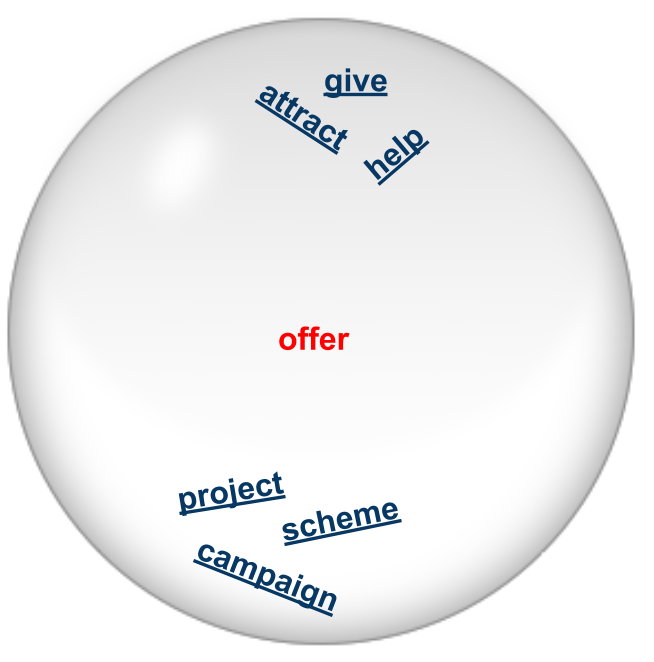
\includegraphics[width=0.5\columnwidth]{sphere.png}
%% %%     }
%% %%   \end{minipage}
%% %%   \caption{The figure on the left presents the input sentences and the randomly
%% %%     sampled substitutes of the word {\em offer} in each sentences.   The right
%% %%   one presents the final embeddings on a representative sphere after S-CODE
%% %%   converges.}
%% %%   \label{fig:scodeexample}
%% %% \end{figure}
%% 
%% The co-occurrence data in Figure~\ref{fig:scodeexample} consists of
%% pairs such as (\textit{W:director}, \textit{S:chairman}) and
%% (\textit{W:chief}, \textit{S:chairman}) therefore S-CODE forces the
%% embeddings of \textit{W:director} and \textit{W:chief} to be close to
%% the embedding of \textit{S:chairman}.  Similarly the embeddings of
%% \textit{W:Pierre} and \textit{W:Frank} will be close to the embedding
%% of \textit{S:John} because they are frequently co-occurring pairs.  As
%% a result the final embeddings of \textit{W:director} and
%% \textit{W:chief} will be close to each other due to the common
%% substitute \textit{S:chairman} and will be apart from
%% \textit{W:Pierre} and \textit{W:Frank} due to the lack of common
%% substitutes (similarly the embeddings of \textit{W:Pierre} and
%% \textit{W:Frank} will be close to each other due to \textit{S:John}).
%% 
%% The coordinates of the embeddings for each unique word and substitute
%% constitute the input to the clustering stage as described in the next
%% subsection.
%% 
%% % How we relate final embeddings and the input pairs?
%% %% S-CODE constructs embeddings on an $n$-dimensional sphere for each word
%% %% type and substitute.  Each pair in the co-occurrence data can be
%% %% represented in three different ways by using the output of S-CODE: (1)
%% %% word embedding (${\bf W}$) which represents the word type information,
%% %% (2) substitute embedding (${\bf C}$) which represents the context
%% %% information, and (3) concatenation of word and substitute embeddings
%% %% (${\bf W}\oplus{\bf C}$).  In the next section we apply k-means
%% %% clustering to these three representation and analyze the
%% %% characteristic of final clusters.
%% 
%% \subsection{Clustering}
%% \label{sec:clustering}
%% %% In Section~\ref{sec:cooc} we describe the transformation of an input
%% %% sentence to a co-occurrence data and we represent each target word
%% %% with the word--substitute pair(s).  In the previous section we
%% %% construct embeddings for each value observed in the co-occurrence data
%% %% using the S-CODE algorithm. 
%% 
%% At this stage, each unique word in the text and each unique substitute
%% sampled to represent their contexts is mapped to a real vector
%% embedding on an $n$ dimensional sphere\footnote{In fact many words
%%   that appear in the text also appear as substitutes and thus get two
%%   embeddings.}.  We apply the instance weighted k-means clustering
%% algorithm to three different representations derived from these
%% embeddings, each with its own advantages and disadvantages:
%% 
%% \paragraph{Type Based:} 
%% In this clustering, each target word {\em type} has a single embedding, and gets
%% assigned to a single cluster.  Clustering word embeddings was previously
%% explored in \cite{yatbaz-sert-yuret:2012:EMNLP-CoNLL}, which achieved the best
%% results to date (80\% \mto) for English.  Sections~\ref{sec:typevsinstance}
%% summarize these experiments for completeness.  
%% %% \paragraph{Clustering substitute embeddings (${\bf S}$)}  
%% %% In a second set of experiments, we ignore target word embeddings and
%% %% apply clustering only to substitute embeddings, associating each
%% %% substitute with a unique cluster.  We then categorize target word {\em
%% %%   tokens} based on what cluster the majority of their substitutes
%% %% belong.  It is important to note that in this setting we are ignoring
%% %% the identity and features of the target words and in effect clustering
%% %% word contexts (substitutes are determined by the context and are
%% %% conditionally independent of the target word).
%% %% 
%% %% For example, the target word {\it W:board} in Table~\ref{tab:samples}
%% %% will be represented with the embeddings of {\it S:board}, {\it
%% %%   S:company} and {\it S:firm} while another occurrence of the word
%% %% {\it W:board} in a different context might be represented with
%% %% embeddings of different substitutes such as {\it S:embark} or {\it
%% %%   S:enter}.  Each occurrence of the target word ``board'' is assigned
%% %% to the cluster in which the majority of its substitute embeddings are
%% %% present\footnote{Ties are broken randomly.}.  This approach generally
%% %% results in higher accuracy for highly ambiguous words like {\em offer}
%% %% where clustering substitute embeddings achieves .82 \mto\ compared
%% %% to the one-tag-per-word upper bound of .74.
%% %% Section~\ref{sec:clustering-s} presents the results of experiments
%% %% clustering substitute embeddings.
%% %% 
%% %% Unfortunately such highly ambiguous words do not constitute a
%% %% significant portion of the corpus and the overall accuracy suffers
%% %% (.64 compared to .80 \mto\ for word clustering).  We also observed
%% %% similar results in our preliminary experiments without S-CODE trying
%% %% to cluster contexts directly (using the Kullback-Leibler divergence
%% %% between their substitute distributions).  Many common words that occur
%% %% in similar contexts and that have similar substitutes, e.g. {\em his}
%% %% and {\em the}, belong to different parts of speech.  In addition,
%% %% words that are generally not substitutable like ``do'' and ``put'' are
%% %% placed in the same category by the PTB.  This suggests that the
%% %% identity and features of the target word are indispensable and that a
%% %% purely substitutability based linguistic definition is insufficient
%% %% for inducing parts of speech as tagged in the PTB.
%% 
%% \paragraph{Instance Based:}
%% In this clustering, we represent each word instance by concatenating the type
%% embedding ($n$ dimensional) with the average of substitutes of that particular
%% instance ($n$ dimensional).  We then apply k-means to the resulting
%% $2n$-dimensional vectors and categorize each instance of a type separately.
%% For instance, the target word ``Pierre'' in Table~\ref{tab:samples} will be
%% represented by concatenating the embedding of {\it W:Pierre} with the average
%% of the embeddings of {\it S:Mr.}, {\it S:Pierre} and {\it S:John}.  This model
%% do not employ the one-tag-per-word assumption and clusters word instances
%% therefore it handles ambiguity.  Clusters that are constructed according to
%% this representation tend to assign fewer categories to each word type than
%% substitute clustering due to the concatenation of ${\bf W}$.  The advantage in
%% highly ambiguous words is still retained (e.g. the \mto\ for {\em offer} is
%% .XX) and the overall result is comparable compared to clustering of word
%% embeddings.  Section~\ref{sec:instance} presents results of the instance based  
%% clustering.
%% 
%% \paragraph{Summary} The first clustering applies the one-tag-per-word
%% assumption from the beginning and clusters word types instead of instances. 
%% %The second setting clusters word contexts (as represented by
%% %substitutes) and is able to categorize individual word tokens.
%% %However it ignores the identity of the target word.  
%% The second one clusters word instances by representing each instance with the
%% concatenation of the word type and average of corresponding substitute
%% embeddings.  The target word is represented without enforcing the
%% one-tag-per-word assumption improves the results on highly ambiguous words
%% while achieving close results with the state-of-the-art system.
%% Section~\ref{sec:exp} compares the performance of these two clustering on the
%% part of speech induction problem, as well as
%% experiments with different features and languages.
